%
% Cost Vector Analysis
%

\section{Quantum cost vector analysis} \label{sec:quantum_meas_cost}
\index{Costs}\index{Attributes}\index{Cost vector analysis}

\dropcap{A}{s} with the classical case in Sec.~\ref{sec:costs}, there will be costs associated with the links and nodes in a network -- nothing is free! In the quantum case, all the usual classical costs are valid, but there are some very important additions of far greater relevance to most quantum applications. Classical digital data is discretised, resulting in data transmission highly robust against noise. In a quantum setting this is necessarily not the case, as the coefficients in quantum superpositions are continuous, meaning that errors accumulate during transmission and states will inevitably deteriorate, unlike digital states. This requires a rethinking of appropriate cost metrics.

%
% Costs
%

\subsection{Costs}

We now briefly introduce some of the key measures for quantifying the quality of quantum communications links, and how they may be expressed as metrics with meaningful operational interpretations. Many of the measures typically employed for characterising quantum systems are not true metrics (i.e costs), but in many cases can be converted to metrics, or used meaningfully as attributes instead.

%
% Efficiency
%

\subsubsection{Efficiency} \index{Loss channel}

The efficiency measure introduced previously is multiplicative, so for consecutive lossy channels the net efficiency is,
\begin{align}
\eta_\mathrm{net}=\prod_i \eta_i,
\end{align}
where $\eta_i$ is the efficiency of the $i$th channel. Intuitively, this is simply telling us that if a photon passes through a channel with success probability $\eta_1$, followed by another with $\eta_2$, the total success probability is \mbox{$\eta_1\eta_2$}.

When employing single-photon encoding of qubits (e.g using the polarisation degree of freedom), there are three basis states of interest: a single photon horizontally polarised ($\ket{H}$); a single photon vertically polarised ($\ket{V}$); and, the vacuum state ($\ket{0}$). The effect of the loss channel on this type of state is to map $\ket{H}$ and $\ket{V}$ to $\ket{\mathrm{0}}$ with probability \mbox{$1-\eta$}, while doing nothing to $\ket{\mathrm{0}}$. Note that because the loss process affects both logical basis states ($\ket{H}$ and $\ket{V}$) identically, its action is invariant under unitary operations in the logical (i.e polarisation) basis space.

%
% Spectral filtering
%

\subsubsection{Spectral filtering} \index{Loss channel}\index{Spectral filtering}

Because spectral filtering can be regarded as a frequency-dependent loss channel, its associated cost can be treated in the same manner, except that rather than keeping track of a single efficiency $\eta$, we track a frequency response function $\eta_f(\omega)$, with the same multiplicative property,
\begin{align}
	\eta_f^\mathrm{(net)}(\omega)=\prod_i \eta_f^{(i)}(\omega).
\end{align}

If we are keeping track of the frequency response, the usual efficiency metric can be made redundant and absorbed into the frequency response function as a uniform response,
\begin{align}
	\eta_f(\omega)=\eta\,\,\forall\,\omega.
\end{align}

%
% Decoherence
%

\subsubsection{Decoherence} \index{Dephasing channel} \index{Depolarising channel} \index{Decoherence}

The dephasing and depolarising channels, given by Eqs.~(\ref{eq:dephasing_channel},\ref{eq:depolarizing_channel}), also behave multiplicatively. If $p_i$ is the probability that the state passing through the $i$th channel in series does not undergo the error process, then the probability of the state passing though the entire series without error is simply,
\begin{align}
p_\mathrm{net}=\prod_i p_i,
\end{align}
exhibiting the same multiplicative behaviour as the loss channel. The same observation applies to any of the other Pauli error channels.

%
% Mode-Mismatch
%

\subsubsection{Mode-mismatch} \index{Mode-mismatch}

In Sec.~\ref{sec:MM_error} we introduced a simple model for temporal mode-mismatch as a displacement in the temporal wave-function of photons propagating through a channel. Clearly, such a process is cumulative -- a temporal displacement of $\Delta_1$ followed by another of $\Delta_2$ yields a net displacement of \mbox{$\Delta_1+\Delta_2$}. Thus, for a chain of such channels we simply accumulate a net temporal displacement of,
\begin{align}
\Delta_\mathrm{net} = \sum_i \Delta_i.
\end{align}

For an incoherent mode-mismatching process, such as time-jitter, an upper bound on the accumulated mismatch may be obtained by summing the maximum temporal displacements at each step.

%
% Distance Measures
%

\subsubsection{Distance measures} \label{sec:fid_metric} \index{Distance measures}

The fidelity of two states directly quantifies how close they are to one another in a geometric sense, i.e on the Bloch sphere \cite{???}, or, in the context of a state passing through a quantum channel, a measure of how well the state is preserved.

The fidelity\index{Fidelity} between two states is defined as,
\begin{align}
\mathcal{F}(\hat\rho_1,\hat\rho_2) = \mathrm{tr}\left(\sqrt{\hat\rho_1^{1/2}\cdot\hat\rho_2\cdot\hat\rho_1^{1/2}}\right),
\end{align}
where,
\begin{align}
& \mathcal{F}(\hat\rho_1,\hat\rho_2) = \mathcal{F}(\hat\rho_2,\hat\rho_1), \nonumber \\
& 0\leq \mathcal{F}(\hat\rho_1,\hat\rho_2) \leq 1.
\end{align}
\mbox{$\mathcal{F}(\hat\rho_1,\hat\rho_2)=1$} iff the states are equal, and \mbox{$\mathcal{F}(\hat\rho_1,\hat\rho_2)=0$} iff they are orthogonal.
In the case where one of the states is a pure state, this simplifies to,
\begin{align}
\mathcal{F}(\hat\rho_1,\ket{\psi_2}) = \bra{\psi_2}\hat\rho_1\ket{\psi_2},
\end{align}
and when both states are pure to simply,
\begin{align}
\mathcal{F}(\ket{\psi_1},\ket{\psi_2}) = |\langle\psi_1 | \psi_2\rangle|^2.
\end{align}

The fidelity is invariant under a common unitary applied to both states,
\begin{align}
\mathcal{F}(\hat\rho_1,\hat\rho_2) = \mathcal{F}(\hat{U}\hat\rho_1 \hat{U}^\dag,\hat{U} \hat\rho_2\,\hat{U}^\dag).
\end{align}

We define the fidelity of two processes, the process fidelity \index{Fidelity} \cite{bib:Gilchrist05}, to be the fidelity between two identical copies of a state that have been evolved under each of those processes, minimised over all possible states. That is, it provides a lower bound on the fidelity between identical states evolved under the two processes. In the context of networking, where quality must be guaranteed, this definition is more appropriate than, say, the average case fidelity. Specifically,
\begin{align}
\mathcal{F}(\mathcal{E}_1,\mathcal{E}_2) = \mathrm{tr}\left( \sqrt{\chi_1^{1/2}\cdot\chi_2\cdot\chi_1^{1/2}}\right),
\end{align}
where $\chi_1$ and $\chi_2$ are the process matrices\index{Process matrices} for $\mathcal{E}_1$ and $\mathcal{E}_2$.

The fidelity of two processes is invariant under a common unitary applied to both channels before or after the process. Specifically,
\begin{align}
\mathcal{F}(\mathcal{E}_1,\mathcal{E}_2) &= \mathcal{F}(\mathcal{E}_U\circ\mathcal{E}_1,\mathcal{E}_U\circ\mathcal{E}_2) \nonumber \\
&= \mathcal{F}(\mathcal{E}_1\circ \mathcal{E}_U,\mathcal{E}_2\circ \mathcal{E}_U),
\end{align}
where $\mathcal{E}_U$ is an arbitrary unitary process.

In the special case of an identity channel, $\hat{\mathbb{I}}$, which is of special interest in many communications scenarios, we employ the shorthand,
\begin{align}
\mathcal{F}(\mathcal{E}) = \mathcal{F}(\mathcal{E},\hat{\mathbb{I}}) = \min_{\hat\rho} \left[\mathcal{F}(\hat\rho,\mathcal{E}(\hat\rho))\right].
\end{align}
By definition \mbox{$\mathcal{F}(\mathcal{E})=1$} iff \mbox{$\mathcal{E}=\hat{\mathbb{I}}$}.

A lower bound on the process fidelity of multiple processes in series is multiplicative,
\begin{align}
\mathcal{F}(\mathcal{E}_2\circ\mathcal{E}_1,\mathcal{E}_3) &\geq \mathcal{F}(\mathcal{E}_2,\mathcal{E}_3)\cdot\mathcal{F}(\mathcal{E}_1,\mathcal{E}_3), \nonumber \\
\mathcal{F}(\mathcal{E}_2\circ\mathcal{E}_1) &\geq \mathcal{F}(\mathcal{E}_2)\cdot\mathcal{F}(\mathcal{E}_1).
\end{align}

Generalising to a sequence of $n$ processes in series yields,
\begin{align}
\mathcal{F}(\mathcal{E}_n\circ\dots\circ\mathcal{E}_1) \geq \prod_{i=1}^n \mathcal{F}(\mathcal{E}_i).
\end{align}

An alternate measure for the distance between two quantum states is the trace-norm distance\index{Trace-norm distance}, defined as,
\begin{align}
D(\hat\rho_1,\hat\rho_2) &= \frac{1}{2}\|\hat\rho_1 - \hat\rho_2\|_1 \nonumber\\
&= \frac{1}{2}\sum_i |\lambda_i|,
\end{align}
where $\lambda_i$ are the eigenvalues of \mbox{$\hat\rho_1-\hat\rho_2$}. Like the fidelity, the trace-norm distance is invariant under unitary transformation. Furthermore, it is contractive under the action of quantum processes,
\begin{align}
D(\mathcal{E}(\hat\rho_1),\mathcal{E}(\hat\rho_2)) \leq D(\hat\rho_1,\hat\rho_2).
\end{align}
The trace-norm distance relates to the fidelity according to the following bounds,
\begin{align}
1-F(\hat\rho_1,\hat\rho_2) \leq D(\hat\rho_1,\hat\rho_2) \leq \sqrt{1-F(\hat\rho_1,\hat\rho_2)^2}.
\end{align}

%
% Purity
%

\subsubsection{Purity} \index{Purity}

The purity of a state that was initially pure quantifies how well quantum coherence was maintained during evolution, equivalently how well superpositions are maintained. The purity is defined as,
\begin{align}
\mathcal{P}(\hat\rho) = \mathrm{tr}(\hat\rho^2),
\end{align}
where,
\begin{align}
\frac{1}{\mathrm{dim}(\hat\rho)} \leq \mathcal{P}(\hat\rho) \leq 1.
\end{align}
We have \mbox{$\mathcal{P}(\hat\rho) = 1$} iff \mbox{$\hat\rho=\ket{\psi}\bra{\psi}$} is a pure state, and \mbox{$\mathcal{P}(\hat\rho)=1/\mathrm{dim}(\hat\rho)$} iff \mbox{$\hat\rho=\mathbb{\hat{I}}/\mathrm{dim}(\hat\rho)$} is the maximally mixed state.

The purity is invariant under unitary operations,
\begin{align}
\mathcal{P}(\hat\rho) = \mathcal{P}(\hat{U}\hat\rho\,\hat{U}^\dag).
\end{align}

The purity of a process is defined analogously to the fidelity of a process,
\begin{align}
\mathcal{P}(\mathcal{E}) = \mathrm{tr}(\chi^2),
\end{align}
and as with the fidelity, a lower bound on the purity of multiple processes in series is multiplicative,
\begin{align}
\mathcal{P}(\mathcal{E}_2\circ\mathcal{E}_1)
\geq \mathcal{P}(\mathcal{E}_2)\cdot\mathcal{P}(\mathcal{E}_1).
\end{align}
\comment{CHECK THIS!}. If the channel implements a unitary operation then necessarily \mbox{$\mathcal{P}(\mathcal{E})=1$}.

Like the process fidelity, the purity of a quantum process is invariant under unitary operations,
\begin{align}
\mathcal{P}(\mathcal{E}) &= \mathcal{P}(\mathcal{E}_U\circ\mathcal{E}) \nonumber \\
&= \mathcal{P}(\mathcal{E}\circ\mathcal{E}_U).
\end{align}

Generalising to a sequence of $n$ processes in series yields,
\begin{align}
\mathcal{P}(\mathcal{E}_n\circ\dots\circ\mathcal{E}_1) \geq \prod_{i=1}^n \mathcal{P}(\mathcal{E}_i).
\end{align}

%
% Entanglement
%

\subsubsection{Entanglement} \label{sec:ent_meas} \index{Entanglement measures}

When distributing entanglement between separate nodes, metrics quantifying bipartite entanglement are relevant. For pure bipartite states $\ket{\psi}_{A,B}$, the purity of one of the reduced subsystems directly quantifies the degree of entanglement between them,
\begin{align}
\mathcal{M}(\ket{\psi}_{A,B})) &= \mathcal{P}(\mathrm{tr}_A(\ket{\psi}_{A,B})) \nonumber \\
&= \mathcal{P}(\mathrm{tr}_B(\ket{\psi}_{A,B})),
\end{align}
The entanglement between two systems in invariant under local unitaries,
\begin{align}
\mathcal{M}(\ket{\psi}_{A,B}) = \mathcal{M}([\hat{U}_A\otimes \hat{U}_B]\ket{\psi}_{A,B}).
\end{align}

%
% Phase-Space
%

\subsubsection{Phase-space} \index{Phase-space errors}

Displacements in phase-space accumulate additively, up to a phase-factor. Specifically, the composition of two displacements is given by,
\begin{align}
\hat{D}(\alpha)\hat{D}(\beta) = e^{\frac{1}{2}(\alpha\beta^*-\alpha^*\beta)}\hat{D}(\alpha+\beta).
\end{align}
Thus, the composition of a chain of unwanted or uncertain displacements yields, up to phase, a displacement with amplitude given by the sum of the individual displacement amplitudes.

Similarly, from the definition of the squeezing operator,
\begin{align}\label{eq:sq_op}
\hat{S}(\xi) = \exp\left[ \frac{1}{2}(\xi^*\hat{a}^2 - \xi{\hat{a}^{\dag 2}})\right],
\end{align}
it is evident that squeezing accumulates additively as well,
\begin{align}
\hat{S}(\xi_1)\hat{S}(\xi_2) = \hat{S}(
\xi_1+\xi_2).	
\end{align}

%
% Channel Capacity
%

\subsubsection{Channel capacity} \label{sec:channel_cap} \index{Channel capacity}

The measures considered until now have quantified the preservation of quantum states. Alternately, one might consider information theoretic measures, which quantify the number of bits/qubits transmitted by a link, i.e the number of bits/qubits in common before and after the channel. This is an extremely powerful tool as it upper bounds the amount of information the receiver can extract from the transmitter under \textit{any} measurement scheme, very useful in a cryptographic context, where we want security to be attack-independent\index{Information-theoretic security} (Sec.~\ref{sec:comp_vs_inf_th_sec}).

The Shannon entropy \cite{???} of a classical probability distribution $X$ is given by,
\begin{align}\index{Shannon entropy}
H(X) = -\sum_x p_x\log_2(p_x),
\end{align}
where $p_x$ are the probabilities in the distribution. For a joint distribution over $X$ and $Y$ this simply generalises to,
\begin{align}\index{Joint Shannon entropy}
H(X,Y) =  -\sum_{x,y} p_{x,y}\log_2(p_{x,y})
\end{align}

The von Neuman entropy \cite{???} for quantum density operators, $S(\hat\rho)$, is defined analogously, replacing probabilities with density operator eigenvalues,
\begin{align}\index{von Neuman entropy}
S(\hat\rho) &= - \sum_x \lambda_x \log_2 (\lambda_x) \nonumber \\
&= -\mathrm{tr}(\hat\rho\,\log \,\hat\rho),
\end{align}
where $\{\lambda\}$ is the eigenvalue spectrum of $\hat\rho$. This modification is logically justified, as the eigenvalues can be interpreted directly as a purely classical probability distribution of orthogonal states when the density operator is transformed into a basis with no coherences between basis states (i.e a diagonal basis or spectral decomposition). In that case the Shannon and von Neuman entropies essentially have identical physical interpretations.

The \textit{mutual information} specifies the number of bits in common between two distributions. Equivalently, it is the maximum number of bits that one party can learn about the other. For two classical distributions, $A$ and $B$, this is given by,
\begin{align}\index{Mutual information}
I(A;B) = H(A) + H(B) - H(A,B).
\end{align}
Equivalently, for density operators,
\begin{align}
I(\hat\rho_A;\hat\rho_B) = S(\hat\rho_A) + S(\hat\rho_B) - S(\hat\rho_A,\hat\rho_B),
\end{align}
using the von Neuman entropy. The mutual information between two quantum states is invariant under local unitary transformations,
\begin{align}
I(\hat\rho_A;\hat\rho_B) = I(\hat{U}_A\hat\rho_A \hat{U}_A^\dag; \hat{U}_B\hat\rho_B \hat{U}_B^\dag),
\end{align}
since the eigenvalue spectrum of a density operator is invariant under unitary transformations. Therefore, the mutual information represents the maximum amount of information Bob can learn about Alice's state under \textit{any} local operations.

A quantum process cannot increase the mutual information between two parties. This yields the \textit{data processing inequality}\index{Data processing inequality} that, for a sequence of channels \mbox{$X\to Y\to Z$},
\begin{align}\index{Data processing inequality}\label{eq:data_proc_ineq}
I(X:Z)&\leq I(X:Y), \nonumber \\
I(X:Z)&\leq I(Y:Z),
\end{align}
with equality if and only if the channel not specified in the identity on the right hand side (\mbox{$Y\to Z$} or \mbox{$X\to Y$} respectively) is unitary, i.e one of the links in the chain perfectly preserves information content. The progression is shown in Fig.~\ref{fig:data_proc_ineq}.

\begin{figure}[!htbp]
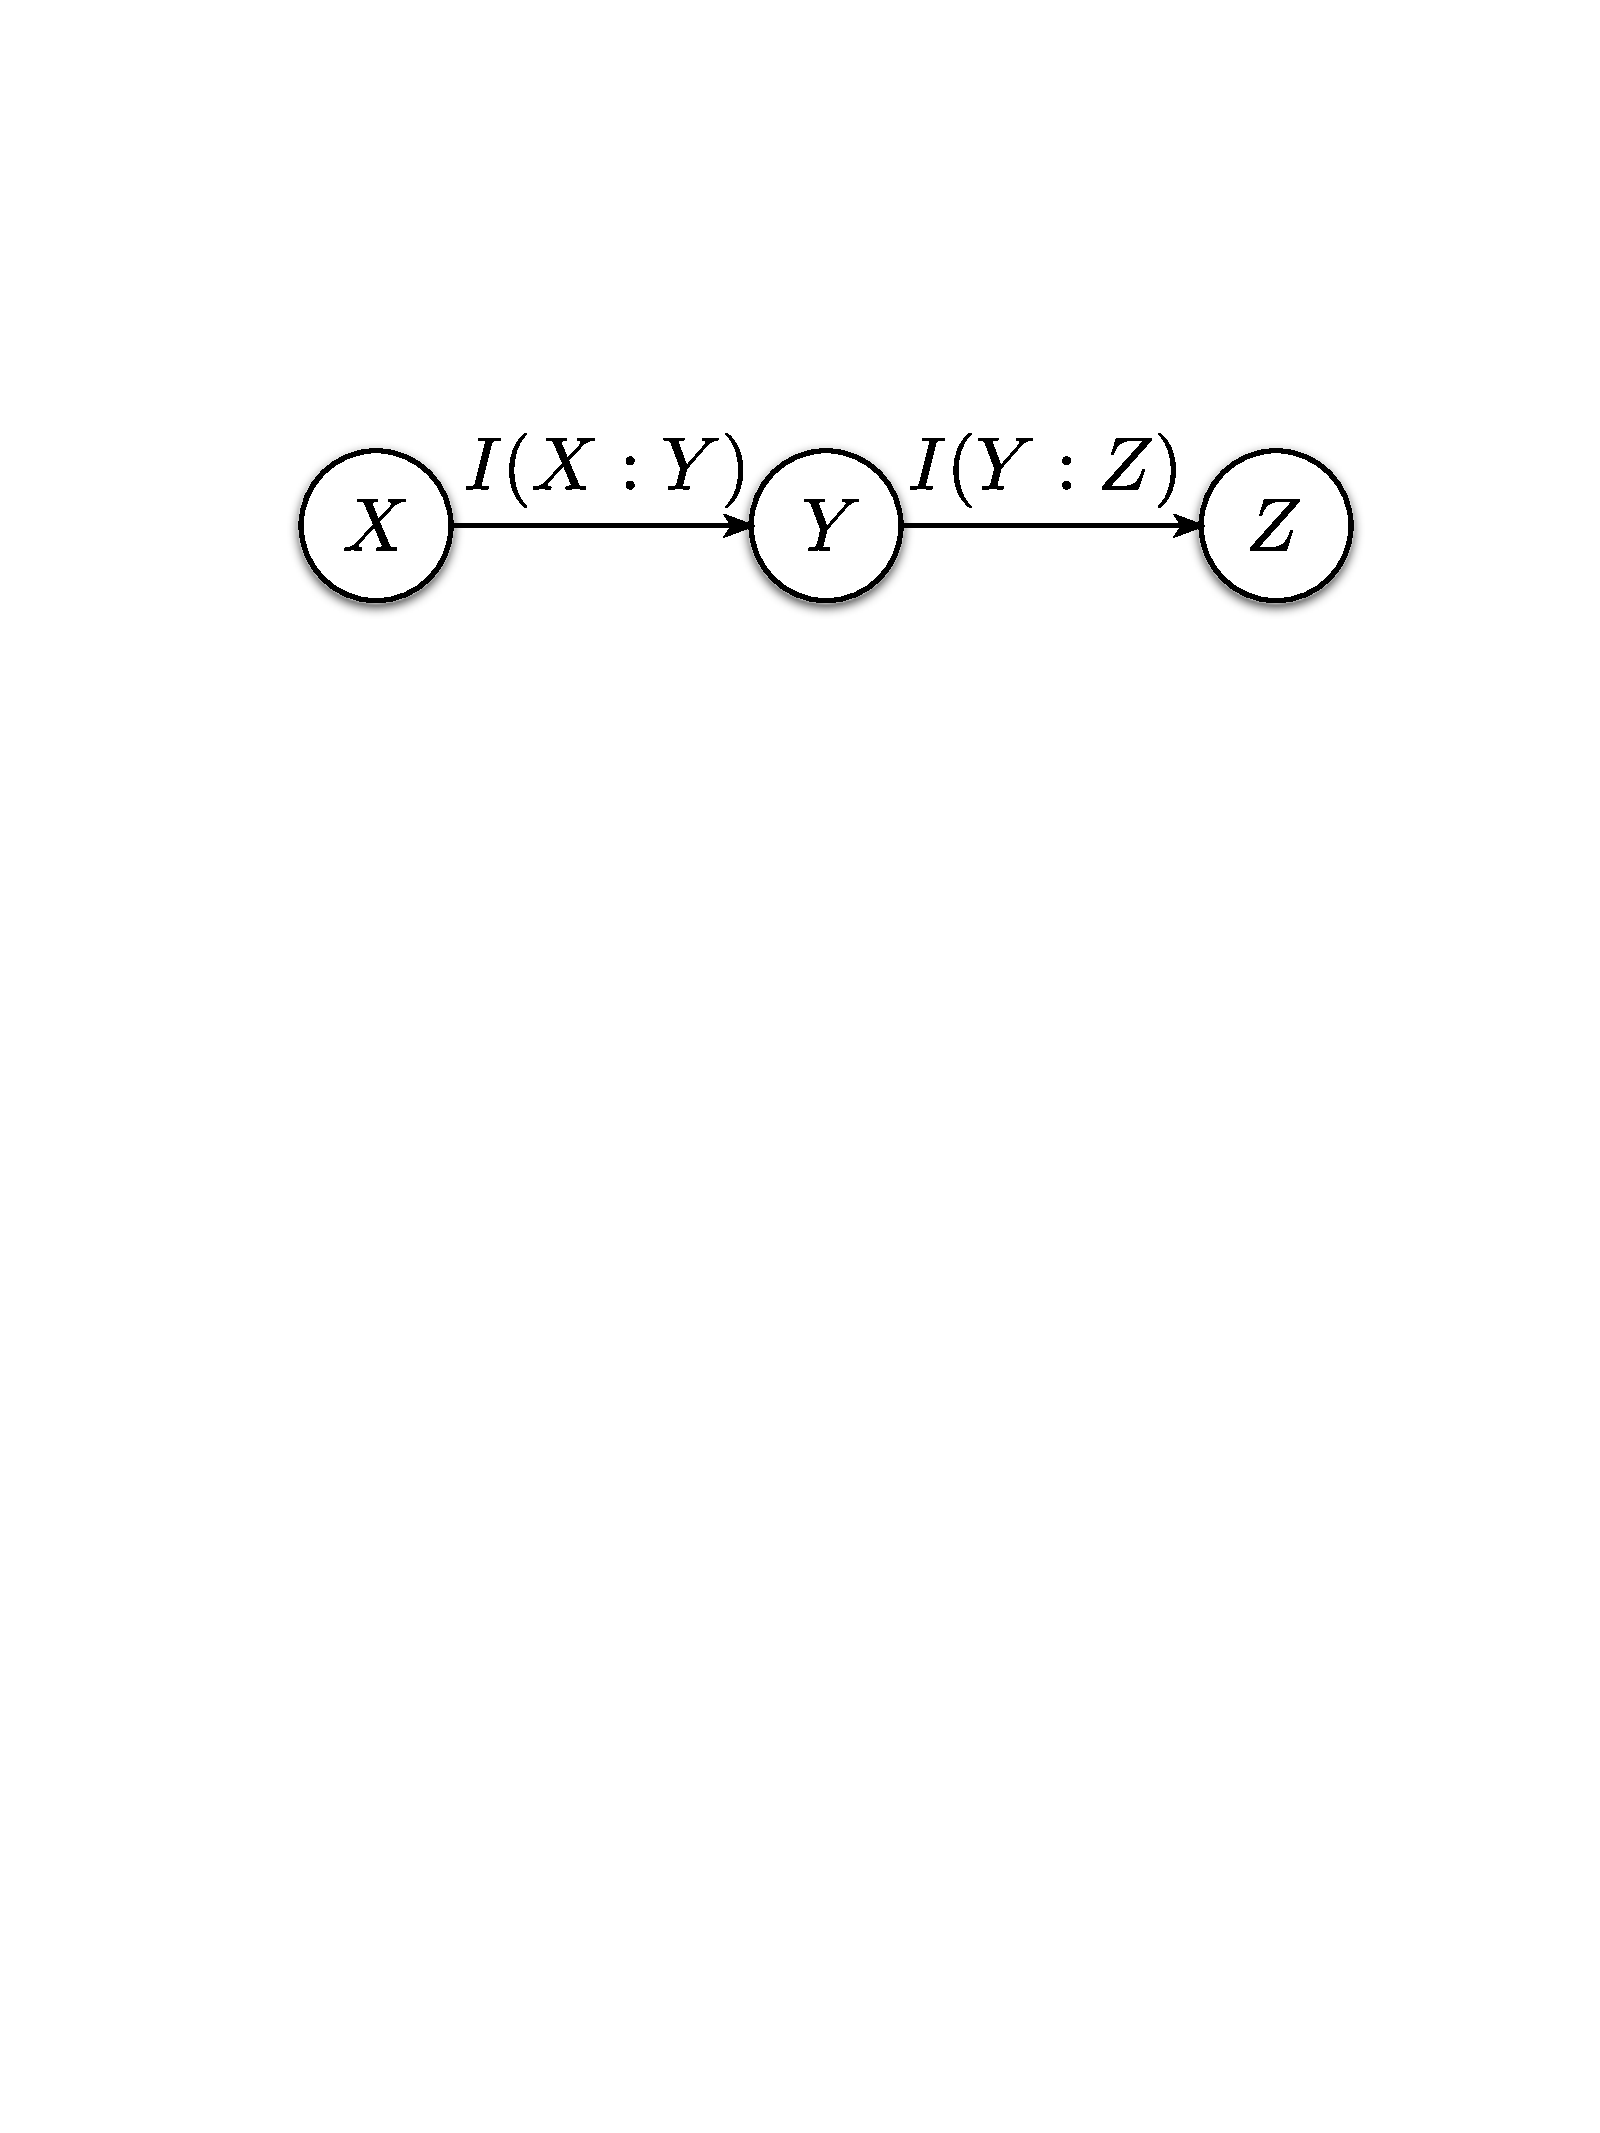
\includegraphics[width=0.3\textwidth]{data_proc_ineq}
\caption{A sequence of events \mbox{$X\to Y\to Z$}. The data processing inequality states that the mutual information from beginning to end is upper-bounded by the mutual information between neighbouring stages, as per Eq.~(\ref{eq:data_proc_ineq}).}\label{fig:data_proc_ineq}	
\end{figure}

The mutual information is defined as being between a particular known pair of states. Of course, in a quantum network we will seldom know what the states being communicated are and will therefore be unable to directly calculate the mutual information. To address this, the \textit{classical channel capacity}\index{Classical channel capacity} of a channel is defined as,
\begin{align}\index{Channel capacity}
\mathcal{C}(\mathcal{E}) = \max_{\hat\rho} [I(\hat\rho,\mathcal{E}(\hat\rho))],
\end{align}
with the intuitive interpretation as the maximum mutual information between input and output states that can be achieved for the channel. (Note: this definition of `capacity' is not to be confused with that which we later refer to in flow networks).

Analogous to the mutual information for classical systems is the \textit{coherent information} for quantum systems \cite{bib:PhysRevA.54.2629}, defined as,
\begin{align}\index{Coherent information}
I(\hat\rho,\mathcal{E}) = S(\mathcal{E}(\hat\rho)) - S_e(\hat\rho,\mathcal{E}).
\end{align}
Here $S_e$ is the \textit{exchange entropy}, a measure of how much information is exchanged between the state $\hat\rho$ and the environment under the action of the process. Specifically, it is given by the entropy of the environment subsystem in Eq.~(\ref{eq:proc_environment}), after application of the channel. This yields the intuitive interpretation that the coherent information is the information contained in the evolved state, discounted by the amount lost to the environment.

The quantum coherent information exhibits much of the same mathematical structure as the classical mutual information. And analogously, we can define the \textit{quantum channel capacity} as,
\begin{align}\index{Quantum channel capacity}
\mathcal{Q}(\mathcal{E}) = \max_{\hat\rho} I(\hat\rho,\mathcal{E}).
\end{align}

Analytic solutions to $\mathcal{C}(\mathcal{E})$ and $\mathcal{Q}(\mathcal{E})$ are not known even for simple Pauli error channels such as dephasing and depolarisation. However, once net dephasing or depolarisation rates have been calculated across a route, the channel capacities can easily be solved numerically, which is sufficient for the numerical algorithms we will rely upon, where a number representing \textit{cost}, rather than an analytic solution, is all we need.

\comment{Add stuff on channel capacities of different channels, like Pauli error channels etc.}

%
% Latency
%

\subsubsection{Latency} \label{sec:latency_metric} \index{Latency}

Aside from the actual information content of a transmitted quantum state, the latency associated with its transmission is a key consideration in many time-critical applications.

By defining the latency of a link/node as the time between receipt of a quantum state and its retransmission, the total latency of a route is simply the sum of all the individual node and link latencies across the route,
\begin{align}
\mathcal{L}(R) = \sum_{i\in R} \mathcal{L}_i,
\end{align}
where $\mathcal{L}_i$ is the latency associated with the $i$th link in route $R$.

%
% Dollars
%

\subsubsection{Dollars} \label{sec:dollars} \index{Dollar cost}

Not to be overlooked is the actual dollar cost of communicating information. It is unlikely that Alice and Bob outright own the entire infrastructure of particular routes. Rather, different links and nodes are likely to be owned by different operators (particularly in ad hoc networks), who are most likely going to charge users for bandwidth in their network (quantum networks won't be cheap). Clearly dollar costs are additive over the links and nodes within routes,
\begin{align}
\mathcal{C}(R) = \sum_{i\in R} \mathcal{C}_i,
\end{align}
where $\mathcal{C}_i$ is the dollar cost of utilising the $i$th link in route $R$.

%
% Costs as Distance Metrics
%

\subsection{Costs as distance metrics} \label{sec:cost_as_dist} \index{Cost distance metrics}

Def.~\ref{def:metric} defines the properties of a cost metric in the classical context. We now wish to consider this in the quantum context.

If we consider a lossy photonic channel for example, efficiencies ($\eta$) are multiplicative -- for a route \mbox{$v_1\to v_2\to v_3$}, the net efficiency is given by the product of the individual efficiencies, \begin{align}
\eta_{v_1\to v_2 \to v_3} = \eta_{v_1\to v_2} \eta_{v_2\to v_3}.
\end{align}
This is multiplicative rather than additive, clearly not satisfying our definition for a cost metric. However, multiplicative metrics\index{Multiplicative metrics} such as this can easily be made additive\index{Additive metrics} by shifting to a logarithmic scale, since
\begin{align}\index{Logarithmic scale}
\log(\eta_{v_1\to v_2\to v_3}) = \log(\eta_{v_1\to v_2}) + \log(\eta_{v_2\to v_3}),
\end{align}
which now has a legitimate interpretation as a distance. The same applies to, for example, frequency response functions, which are equivalent to frequency-dependent loss.

In general, for a series of links \mbox{$v_1\to v_2 \to \dots \to v_n$} characterised by multiplicative measure $m$, the equivalent cost metric is,
\begin{align} \label{eq:dist_log}\index{Logarithmic distance}
c_{v_1\to v_2 \to \dots \to v_n} = -\sum_{i=1}^{n-1} \log (m_{v_i\to v_{i+1}}).
\end{align}
We have assumed that \mbox{$0\leq m \leq 1$}, where \mbox{$m=0$} represents complete failure, and \mbox{$m=1$} represents ideal operation.

With these properties, the costs in our graph have an elegant interpretation. In the case of perfect operation, \mbox{$m=1$}, the cost is \mbox{$c=0$}, creating an ideal direct link between neighbouring nodes at no cost. On the other hand for complete failure, \mbox{$m=0$}, the cost metric is \mbox{$c=\infty$}, effectively removing the link from the network and prohibiting pathfinding algorithms from following that route altogether.

Such a logarithmic scale is particularly convenient when a cost metric over links accumulates on a per physical distance basis, in which case the cost metric is simply the physical length of the link multiplied by the metric per unit distance. For example, if a fibre channel implements loss at 3dB/km, the loss over 10km is 10$\times$3dB.

Note that lower bounds on fidelity, purity, efficiency and dephasing are all multiplicative on a scale of 0 to 1, and thus their logarithms may be regarded as cost metrics. Spatio-temporal mode-mismatch, latency, dollar cost and displacements are clearly automatically metrics as they are additive.

A dephasing channel can be easily converted to a distance metric as follows. First we reparameterise the dephasing channel into,
\begin{align}
\mathcal{E}(\hat\rho) &= p\hat\rho + (1-p)\hat{Z}\hat\rho\hat{Z}\nonumber\\
&= (2p-1)\hat\rho + (1-p)(\hat{Z}\hat\rho\hat{Z} + \hat\rho).	
\end{align}
Now \mbox{$2p-1$} is the probability that the state is not dephased and \mbox{$1-p$} is the probability that the state is replaced with the completely dephased state. Therefore the probability of multiple applications of the channel not dephasing the state scales multiplicitavely as\footnote{With this parameterisation, in the limit of many applications of the dephasing channel, an input state asymptotes to the completely dephased state, \mbox{$\lim_{n\to\infty} \mathcal{E}^n(\hat\rho) = \frac{1}{2}(\hat{Z}\hat\rho\hat{Z}+\hat\rho)$}. Thus, \mbox{$2p-1$} can be regarded as a discretised parameterisation of a system's $T_2$-time\index{$T_2$-time}.},
\begin{align}
p_\mathrm{no\, error} = \prod_{i}(2p_i-1),
\end{align}
which is additive in a logarithmic scale as before,
\begin{align}
\log(p_\mathrm{no\, error}) = \sum_i \log(2p_i-1),
\end{align}
which acts as a distance metric. This approach can similarly be applied to other Pauli channels.

In the case of mutual information and channel capacity, it makes most sense to consider the number of bits that are lost by a channel, rather than the number communicated, since then we have a measure with quasi-metric properties. Specifically, let the number of bits lost by a channel be the difference between the number of bits in the input state and the channel capacity,
\begin{align}
B_\mathrm{lost}(\mathcal{E},\hat\rho) = S(\hat\rho) - \mathcal{C}(\mathcal{E}).
\end{align}
Then there are two cases to consider -- upper and lower bounds on accumulated lost bits.

The best-case scenario is that subsequent channels lose the same bits, giving us a lower bound on the number of lost bits as the maximum number of bits lost by the constituent channels,
\begin{align}
B_\mathrm{lower}(\mathcal{E}_2\circ\mathcal{E}_1,\hat\rho) = \mathrm{max}[B_\mathrm{lost}(\mathcal{E}_1,\hat\rho), B_\mathrm{lost}(\mathcal{E}_2,\hat\rho)].
\end{align}
Alternately, each subsequent channel could lose a different set of bits, in which case the number of lost bits accumulates additively,
\begin{align}
B_\mathrm{upper}(\mathcal{E}_2\circ\mathcal{E}_1,\hat\rho) = B_\mathrm{lost}(\mathcal{E}_1,\hat\rho) + B_\mathrm{lost}(\mathcal{E}_2,\hat\rho). 
\end{align}
Then, the number of actual bits lost is bounded from above and below as,
\begin{align}
B_\mathrm{lower} \leq B_\mathrm{lost} \leq B_\mathrm{upper}.	
\end{align}

%In the case of mutual information, which is not a metric, one can use it to define the \textit{variation of information} metric,
%\begin{align}\index{Variation of information}
%d_\mathrm{VI}(X,Y) &= H(X,Y) - I(X;Y), \nonumber \\
%d_\mathrm{VI}(\hat\rho_A,\hat\rho_B) &= S(\hat\rho_A,\hat\rho_B) - I(\hat\rho_A;\hat\rho_B),
%\end{align}
%or for a channel,
%\begin{align}
%d_\mathrm{VI}(\hat\rho,\mathcal{E}) &= S(\hat\rho,\mathcal{E}(\hat\rho)) - I(\hat\rho;\mathcal{E}(\hat\rho)),
%\end{align}
%which obeys the metric properties.

%
% Non-Trivial Node Operations
%

\subsection{Non-trivial node operations}

Thus far we have considered how to accumulate cost metrics across routes through a network, where each link is subject to some quantum process obeying our notion of a cost metric. But what happens when the links are interspersed with nodes that may be doing more than just simple switching?

A more general scenario to consider is where the nodes are not restricted to routing, but can additionally implement arbitrary unitary operations. This substantially broadens the class of networks under consideration, to encompass nodes capable of doing everything from straightforward routing to entire quantum computations.

All of the examples for cost metrics we introduced in Sec.~\ref{sec:quantum_meas_cost} have the property that they are invariant under unitary operations. Therefore the costs along a route may simply be accumulated as before, summing up the edge weights, without needing any special treatment for node operations, provided they are unitary. For non-unitary node processes, we can merge them into their neighbouring link processes as before (see Fig.~\ref{fig:remove_nodes}).

\subsection{Negative cost vectors}\index{Negative cost vectors}

When we initially introduced cost vector analysis in the classical context (Sec.~\ref{sec:costs}) we insisted that costs be positive by definition. However, in the quantum scenario we will loosen this demand since negative costs arise quite naturally in the context of operations that \textit{improve} quantum data. Specifically this arises naturally when nodes implement operations such as entanglement purification or quantum error correction, to be discussed in detail in Sec.~\ref{sec:QOS_chap}. In that case making what would otherwise be a routing detour can yield net benefit, and so the cost vector analysis must take these negative costs into consideration and give them the favourable treatment they deserve.